%!TEX root = ../thesis.tex

\cleardoublepage
\chapter{Background Information and Related Work}
\label{cha:background}

To place this thesis in its proper academic and practical context, this chapter will provide the necessary information on relevant topics as well as reviewing some of the existing approaches in literature which bear similarity or served as an inspiration. First mobile networking and 5G will be discussed, then multipath solutions will be covered and lastly deterministic networking.

\section{Mobile Networks and Backhaul}

The defining characteristic of a mobile network is wireless connectivity. This enables the users to move around while remaining connected to the network, which stands in direct opposition to historical computer networks which were stationary and usually featured fixed connections between computers. A user in a mobile network must first detect and then connect to a Base Station, after which they are authenticated and authorized. A user may be switched from one Base Station to another depending on the signal strength (this is referred to as a handover). All of the user's data sent in the network goes through the Base Station to which it is currently connected. At first this data was exclusively analog voice data, however over time newer versions of the mobile networking specifications have defined different types of data, and eventually Internet Protocol (IP) messages as well. Starting with 4G, mobile networks have transitioned to an all IP architecture \cite{3gpp.36.300}. In order to support and manage this mobility and provide internet connectivity, today's mobile networks have a complex internal architecture where different network functions are responsible for the different aspects of user management.

\begin{figure}[ht]
    \centering
	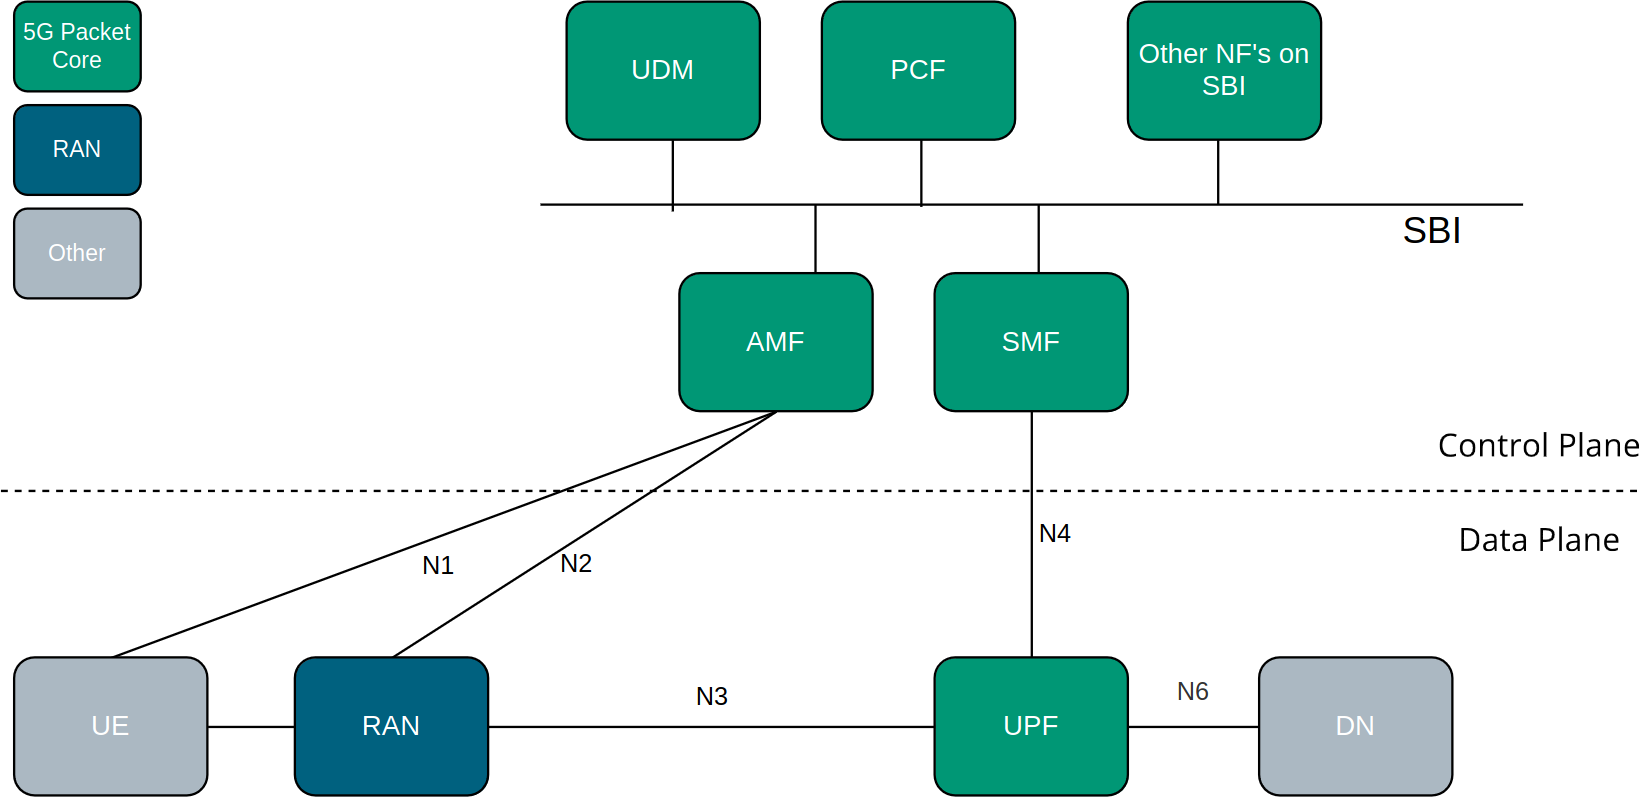
\includegraphics[width=\linewidth]{fig/core.png}
	\caption{Simplified 5G Architecture}
	\label{fig:core}
\end{figure} 

Figure \ref{fig:core} shows a simplified version of the architecture of a 5G core network and how it is connects to the RAN, the user, and the internet. The figure does not include all of the Network Functions defined in the 5G specifications but shows a select few which will be briefly explained in following.

The Access and Mobility Management Function (\textbf{AMF}) handles, among other things, the user registration (access authentication and authorization), connectivity management, and the control plane interface to the RAN. The reference point for interactions between the AMF and the RAN is called the N2 reference point. The protocol used for these interactions is the NGAP protocol. The reference point for interactions with the UE is N1. This is a purely logical interface, messages between the UE and the AMF actually have to physically go through the RAN.

The User Plane Function (\textbf{UPF}) is responsible for forwarding packets between the Data Network and the RAN. The UPF must also perform QoS enforcement, for example making sure users do not exceed the limits of their subscription. The UPF communicates with the RAN over the N3 reference point. For this they utilize the GTP protocol. GTP is a tunneling protocol designed for mobile networks. Packets originating in the RAN are contained in a GTP tunnel and must be de-capsulated by the UPF before being forwarded to the Data Network. Packets in the opposite direction must have a GTP header added to them before they are sent to the RAN.

The Session Management Function (\textbf{SMF}) is responsible for session establishment and management, and it configures traffic steering in the UPF. The SMF and the UPF communicate over the PFCP protocol on the N4 reference point. Their interactions are a lot like those between a switch and a controller in a Software Defined Network.

The Policy Control Function (\textbf{PCF}) provides policy rules to different Control Plane functions in order to enforce them. The SMF consults the PCF in order to pass on the information to the UPF what Quality of Service a given user should experience. The interactions between the SMF and the PCF go over the Service Based Interface (SBI). This is a logical interface which represents all of the different interactions between all of the Control Plane Network Functions. Communication on the SBI uses the http2 protocol.

In the figure it can also be seen how the 5G Core (like the 4G Packet Core before it) splits the control plane and the user plane (or data plane). The network functions in the control plane co-ordinate to make decisions over how to orchestrate the data plane, while the components in the user plane are the ones handling the actual user traffic.

\subsection{Backhaul in 5G}

The first hop from the user equipment (UE) into the mobile network occurs over the air, between the UE and the Base Station, via wireless signals. The network of different Base Stations is called the Radio Access Network (RAN). Once the user has transmitted its data to the RAN, the RAN is responsible for passing on the user's messages to the core network. The transport network between the RAN and the Core is the backhaul network or backbone \cite{jaber20165g}, however the term backhaul can also be used to refer to the process of transporting data from the RAN back to the core.

In light of the increased focus on enabling time sensitive industrial use cases 5G the authors in \cite{prados2021asynchronous} proposed a method for integrating asynchronous Time Sensitive Networking into 5G backhauling. To achieve this their architecture uses an Asynchronous Traffic Shaper, which is crucial for integrating the time sensitive traffic with the regular traffic. Their solution also utilized frame replication for the delay critical flows defined in the 5G specifications (5G QoS Identifiers (5QIs) 82 through 85).

The authors of \cite{jaber20165g} highlight the need for innovation in 5G backhaul provisioning. At present optic fibre backhaul is not available nationwide in Europe, and Fibre to the Home (FTTH) is scarce worldwide. Currently most backhaul networks are built with microwave links or fibre/copper based links. There has also been research \cite{seppanen2016multipath, saadat2018multipath} into using multipath routing within the context of millimeter Wave (mmWave) backhaul in order to increase both reliability and throughput.

TODO: Satellite backhaul

\subsection{5G and Campus Networks}

In order to enable new industrial use cases, 5G campus networks may be deployed exclusively for users within a campus organization, and covering only a prescribed geographical area \cite{rischke20215g}. The deployment of such a network can be crucial for time-sensitive wireless communication, e.g. between robots, and the 5G specifications contain traffic classes and QoS requirements for delay-critical use cases \cite{3gpp.23.501}, this is done in order to make 5G a competitive, or even superior, option to WiFi in campus deployments \cite{walia20175g}.

There is lots of room for different deployment architectures for 5G campus and non-public networks (NPN's). In \cite{prados20215g} many of these architectures are discussed and investigated. In order to operate a 5G campus network, spectrum may need to be acquired, as well as 4G or 5G base stations, depending on the mode of operation- NSA or SA. Furthermore, a 5G Core Network is required in order to manage the network. 5G places an increased focus on virtualization and flexibility of deployment. As such there are a litany of options for which network functions from the core to deploy, and where to deploy them.

This thesis addresses specifically those campus network deployments which require backhaul to a core located off premises. Networks deployed in this fashion will typically feature a subset of the core's network functions deployed on premise. In the simplest case this subset will be the empty set, and the only component on premise will be the RAN. A more common deployment model may feature one UPF on site with a second UPF located in the core, and packets being forwarded between these two UPFs. The WAN Connector will be designed to be able to backhaul IP traffic from the remote campus to the core. This means it can be placed "after" the RAN or "after" the UPF, respectively, in these scenarios ("after" from the perspective of the uplink traffic), in order provide deterministic backhaul for the IP traffic it is forwarding. In the core, the terminating WAN Connector will be placed "before" the UPF.


\section{Multipathing and Multihoming}

At this point it becomes important to establish certain definitions and similar terms, and how they will be used in this thesis. Multihoming refers to a host which has more than one outgoing interface on which it may forward packets for which it does not have a direct link to the destination. A multihomed host may choose to use different links for different traffic. Multipath routing, which may also be called "multipathing"

\subsection{Collecting Link and/or Path Performance Metrics}

In \cite{akella2008performance} the authors collected both passive metrics (looking at response times for outgoing packets), and active measurements (sending ICMP ping, or TCP SYN messages and measuring the response time). Using the passive measurements enabled their multihomed approach to perform well, but when using the active measurements the performance was even better. Crucially, the passive measurements worked better over larger sampling periods, because it took longer to get a full overview of all the possible routes. Whereas the active sampling approach acquired it's measurements faster and was thus more effective over smaller sampling intervals.

Considering these results, the solution developed in this work will therefore utilize both active and passive measurements. All three metrics- packet loss, latency, and jitter- will be periodically measured in an active manner. The period over which to perform these measurements is also an important design decision for the WAN connector, and it will be a fixed value, which can be configured by the operator. The use of a fixed value is important in the context of a solution which aims to provide determinism, since traffic may often have hard requirements for the maxmimum tolerable latency, packet loss, or jitter, which may be experienced within a given window (e.g. in the 5G QoS specifications the averaging window for non delay critical traffic is 2 seconds \cite{3gpp.23.501}).

For classical wired links in multihomed scenarios, \cite{tao2004exploring} have observed that one link will generally dominate with regards to latency, but with brief periods where other links' performance is superior. These same authors also note that with regards to packet loss there is far less prevalence of a "dominant" link, and generally the links will perform comparably. Packet loss is also a particularly difficult metric to measure, since most links are highly reliable and when they do experience packet loss it is in bursts \cite{tao2004exploring}. Wireless connections are usually less reliable and may experience more consistent rates of packet loss at the data link layer, however it is opaque from the perspective of the higher layers, which may only perceive it through the jitter and/or latency.

Ultimately, many of the best performing approaches for predicting packet loss, e.g. Hidden Markov Models \cite{tao2004exploring, bremler2002predicting}, are still somewhat imprecise and inaccurate. These models assume the link is in one of two states, good or bad, and each state has a different probability for packet loss, and there is a transition matrix which represents the probabilities of switching from one state to another.

\subsection{Path and/or Interface Selection}

Interface selection in multi-homed environments, as well as multipath routing are mature and well researched topics. Here, a selection of those approaches which are specifically relevant will be covered.

Wireless Sensor Networks (WSNs) are often deployed in challenging environments and must construct their routing tables dynamically. Research into multipath routing solutions for providing QoS guarantees in WSNs can serve as inspiration for this thesis' approach. In \cite{alwan2010multi}, the authors use Routing Request (RREQ) flooding to build knowledge of disjoint paths. The RREQ's also include a minimum reliability so that the paths found all comply to this requirement. Then when maintaining routing table entries the probability of success is also stored. This information is then used in the path selection. While this approach is good for WSNs, in the context of a 5G campus network it is not feasible because it uses the Ad-hoc On-demand Distance Vector (AODV) Routing \cite{perkins2003rfc3561} protocol, whereas the public internet uses BGP \cite{rekhter2006border}.

A more relevant example is the work in \cite{huang2008multiconstrained}, where the authors also address QoS provisioning in a WSN, using multipath routing. Their approach is to formulate the problem as a probabilistic programming problem and then convert it to a linear programming problem using an approximation technique. When solved, the equation they use to represent the problem yields which paths packets should be sent on (or duplicated on) in order to achieve the desired reliability. Only for those paths which would guarantee the maximum latency is still below the QoS requirements are considered. This approach bears similarity to how \cite{prados2021asynchronous} (discussed earlier) replicates certain flows.

Another article which deserves mentioning is the work in \cite{akella2008performance}. Here, the authors evaluate a large set of route-control mechanisms and evaluate their trade-offs for multihomed enterprises, in order to derive "best common practices" for multihoming. Their most important results shows that there is no benefit to using historical samples, route selection should always be based on current samples. Furthermore they even find that that at times employing historical data to make decisions about which path to forward on can prove detrimental.

%Finally the last work which will be discussed is \ref{rodriguez2004mar}. In this work, the authors built a commuter mobile access router infrastructure which uses multiple wireless service providers. Much like the WSN examples this approach is a wireless multihomed device.

\section{Determinism in Computer Networking}

%\subsection{Quality of Service (QoS)}

\subsection{Deterministic Networking Specification}



\subsection{Traffic Shaping and Bufferbloat}

Since the DetNet specifications explicitly mention the use of a traffic shaper to avoid bufferbloat it is worth exploring what these are and may entail.

First, to bufferbloat; this phenomenon refers to the use of disproportionately sized buffers, and their effect on the latencies experienced when these buffers are full \cite{allman2012comments, gettys2011bufferbloat}. The TCP congestion avoidance algorithm depends on dropped packets in order to detect when the bottleneck link along the path is saturated, and reduce its window size in response. When congested links finally do drop packets, if these packets are the last ones in the queue it means the whole rest of the queue must be sent first before the dropped packets are detected and the window size is reduced. This means that there is an unnatural delay before congestion is detected, and during that period all packets passing through the node experience unnecessary latency due to the congestion induced buffering. This problem has been heavily exacerbated by the cheap availability of memory and the desire for low packet loss. This is a fundamental misunderstanding. Dropping TCP packets is a means of communication and is not at all the same as packet loss which occurs to equipment failure or transmission errors. By dropping packets when a TCP flow exceeds its throughput, congestion is communicated. This problem can occur with UDP as well but it is even harder to detect in those instances.

The first solution to this problem lies in properly sized buffers, another solution includes Early Congestion Notification (ECN), wherein TCP is explicitly warned of congestion in messages instead of through dropped packets. The other solution comes in the form of traffic shaping. Specifically, by using active queue management and fair queuing it is possible to selectively drop packets from a buffer (e.g. only those for a greedy TCP flow) and also dequeue other packets earlier (e.g. a different flow which is not congesting the link). This overcomes the bufferbloat problem by causing the greedy TCP flow to reduce its throughput and letting through those flows that are not using more than their share of the bandwidth.

Beyond mitigating buffer bloat, traffic shaping can still be important for highly latency sensitive applications. Congestion can be avoided by smoothing out any large bursts of packets. Furthermore, traffic shaping is a fundamental design decision that must be made. If a link is to be kept busy at all times, so that maximum throughput is achieved, it means that latency critical packets may not always be forwarded on time. Conversely, by reserving some portion of the bandwidth in case latency sensitive traffic arrives, the full bandwidth cannot be used at all times and thus the throughput is reduced. This is a fundamental trade-off which must be made.





















